\documentclass[conference]{IEEEtran}
\IEEEoverridecommandlockouts
% The preceding line is only needed to identify funding in the first footnote. If that is unneeded, please comment it out.
\usepackage{cite}
\usepackage{amsmath,amssymb,amsfonts}
\usepackage{algorithmic}
\usepackage{graphicx}
\usepackage{textcomp}
\usepackage{xcolor}
\def\BibTeX{{\rm B\kern-.05em{\sc i\kern-.025em b}\kern-.08em
    T\kern-.1667em\lower.7ex\hbox{E}\kern-.125emX}}
\usepackage{comment}
\usepackage{array}
\usepackage{booktabs}
\usepackage{url}
\usepackage{tikz}
\usetikzlibrary{calc,positioning}
\usepackage{adjustbox}

% Short names used throughout the paper
\newcommand{\swinp}{Swin-UNet++-Partial}
\newcommand{\swint}{Swin-P}        % abbreviation used in tables
\newcommand{\degC}{\textdegree{}C}

\begin{document}
\title{Semantic Segmentation of Facial Regions in Thermal Images: A Reproducible Benchmarking Framework for U-Net, TransUNet, and Swin-UNet++
%{\footnotesize \textsuperscript{*}Note: Sub-titles are not captured in Xplore and should not be used}
%\thanks{Identify applicable funding agency here. If none, delete this.}
}

\author{Omitted For Blind Review}

\begin{comment}
\author{\IEEEauthorblockN{1\textsuperscript{st} Given Name Surname}
\IEEEauthorblockA{\textit{dept. name of organization (of Aff.)} \\
\textit{name of organization (of Aff.)}\\
City, Country \\
email address or ORCID}
\and
\IEEEauthorblockN{2\textsuperscript{nd} Given Name Surname}
\IEEEauthorblockA{\textit{dept. name of organization (of Aff.)} \\
\textit{name of organization (of Aff.)}\\
City, Country \\
email address or ORCID}
}
\end{comment}

\maketitle

\begin{abstract}
Isolating anatomical regions is a prerequisite for extracting meaningful temperatures from thermal facial images. 
However, architecture comparisons for this task are often confounded by identity leakage between training and evaluation data, identical hyperparameters imposed across different architectural families, undeclared training budgets, and computational costs measured under unequal conditions. 
We present UBench, an open, end-to-end benchmarking framework for multi-region semantic segmentation of thermal faces, and use it to compare U-Net, TransUNet, and \swinp{} (a simplified Swin-based baseline built for this work) on 10 classes derived from the landmark annotations of the Charlotte-ThermalFace dataset.
The protocol combines subject-disjoint 5-fold cross-validation, a family-specific optimization strategy with an identical 100-epoch budget, and measurements of latency, and peak memory measured under a fixed batch size, along with Wilcoxon signed-rank tests paired by subject. 
TransUNet achieved the highest final-epoch mIoU ($0.433$), followed by U-Net ($0.405$) and \swinp{} ($0.353$); Although all subject-paired comparisons were statistically significant ($p \le 0.0039$, $n=10$), the variability across validation folds ($0.0995$) exceeds the largest gap between architectures ($0.0868$). Furthermore, after excluding four lateralized classes affected by mask-derivation defects, only the advantage of TransUNet remained significant. 
Efficiency reverses the accuracy ordering: \swinp{} processes $89.7$ images/s with $300.6$~MB of inference memory, against $55.6$ and $39.2$ images/s for U-Net and TransUNet. 
We also show how two flawed memory probes produced two opposite memory rankings and report the pipeline audit that exposed them.

%Isolating specific anatomical regions is essential for accurately extracting temperatures from thermal facial images. 
%However, architecture comparisons for this task are often confounded by identity leakage between training and evaluation data, identical hyperparameters imposed across different architectural families, undeclared training budgets, and computational costs measured under unequal conditions. 
%Isolating anatomical regions is a prerequisite for extracting meaningful temperatures from thermal facial images; yet, comparisons between different architectural models for this task are often complicated by several factors, including identity leakage between training and evaluation datasets, the application of the same hyperparameters across different architectural families, undisclosed training budgets, and varying conditions under which computational costs are measured. 

\end{abstract}

\begin{IEEEkeywords}
semantic segmentation, thermal imaging, benchmarking, reproducibility, U-Net, vision transformers
\end{IEEEkeywords}

%==============================================================================
\section{Introduction} \label{sec:introducao}
%==============================================================================

Infrared thermography captures radiation emitted by a surface, which depends on its temperature, and therefore measures skin temperature without contact or external illumination \cite{Nowakowski2025}.
A temperature measurement, however, is only as valid as the region it is averaged over.
Facial temperature is not uniformly distributed across regions that differ in vascular supply, tissue thickness, and sensitivity to ambient conditions: the inner corner of the eye correlates strongly with core temperature, whereas the forehead and cheeks are more susceptible to environmental artifacts \cite{Ioannou2014,Gioia2024}.
Isolating each anatomical region is thus a methodological prerequisite for downstream measurement, and because manual delineation is impracticable frame by frame, it must be automated by semantic segmentation.

Multi-region segmentation of thermal faces remains underexplored: most work targets face detection, landmark localization, or a single region of interest \cite{Vega2025,Chu2019,Jerbi2024}, and thermal segmentation as a whole is a fragmented subfield with heterogeneous evaluation protocols \cite{Kutuk2022}.
More importantly, architecture comparisons in this setting are fragile because of four recurring practices.
(i)~\textbf{Identity leakage}: when frames of the same subject appear in training and evaluation, metrics reward memorization of faces rather than generalization.
(ii)~\textbf{Identical hyperparameters} across convolutional and attention-based families implicitly adopt one family's recipe as the standard and handicap the other.
(iii)~\textbf{Undeclared training budgets} let an architecture look superior merely because it was trained longer.
(iv)~\textbf{Cost measured under unequal conditions}, such as different batch sizes or unsynchronized GPU timers, makes efficiency rankings incomparable.
Isensee et al.~\cite{Isensee2024} argue that much of the progress reported in medical segmentation stems from such validation practices rather than from architectural innovation.

This paper presents \textbf{UBench}, a reproducible benchmarking framework that addresses these four methodological issues by design and uses it to compare U-Net \cite{Ronneberger2015}, TransUNet \cite{Chen2021}, and \swinp{}, a simplified Swin-based baseline, on 10 facial classes of the Charlotte-ThermalFace dataset \cite{Ashrafi2022}.
We answer three research questions:
\textbf{RQ1}: Which architecture achieves the highest accuracy, and is the difference statistically distinguishable from experimental variability?
\textbf{RQ2}: How does per-class performance relate to region size and to the fidelity of the derived reference masks?
\textbf{RQ3}: What is the relationship between accuracy and computational cost under equalized conditions, when cost is measured?

The contributions are:
\begin{itemize}
\item an open, end-to-end benchmarking framework, from radiometric preprocessing to paired statistical analysis, in which all architectures share one training loop, one metric implementation, and one cost-measurement procedure;
\item a benchmark of three architectures under subject-disjoint cross-validation, family-specific recipes, an identical declared budget, and subject-paired significance tests;
\item the empirical finding that, in this domain, the variability across validation partitions exceeds the difference between the best and worst architectures, together with a sensitivity analysis showing that only a \emph{partial} ordering survives the exclusion of classes affected by label defects;
\item a measurement-methodology account, drawn from a 32-item audit of the pipeline, of how silent instrumentation defects reversed the memory ranking twice and corrupted labels without raising any errors.
\end{itemize}

Section~\ref{sec:trab_relac} reviews related work; Section~\ref{sec:metodologia} describes the framework and protocol; Section~\ref{sec:resultados} reports the results; Section~\ref{sec:discussao} discusses them; and Section~\ref{sec:conclusao} concludes. 

%==============================================================================
\section{Related Work} \label{sec:trab_relac}
%==============================================================================

\textbf{Thermal face analysis.}
Most machine-learning work on thermal faces addresses the steps that precede segmentation.
Robledo-Vega et al.~\cite{Vega2025} detect thermal faces with YOLOv8/YOLO11 on embedded platforms, evaluating on Charlotte-ThermalFace; Chu and Liu~\cite{Chu2019} localize thermal facial landmarks with multi-task CNNs; and Kopaczka et al.~\cite{Kopaczka2018} provide the landmark-annotated \textit{Thermal Face Database}.
Studies that estimate body temperature typically rely on a few hand-picked regions; Jerbi et al.~\cite{Jerbi2024}, for instance, use the eye, nose, and cheek, and confirm that the region from which temperature is extracted determines measurement quality.
These works output boxes or coordinates, whereas segmentation assigns a label to every pixel and delimits the area over which temperature statistics are computed.

\textbf{Thermal segmentation.}
The closest work is that of Joshi et al.~\cite{Joshi2022}, who segment thermal faces into multiple regions with self-adversarial multi-scale contrastive learning.
They share three methodological choices with this paper: reference masks derived from anatomical landmarks, a split by subject identity, and the use of absolute per-pixel temperatures instead of per-image normalization.
On the \textit{Thermal Face Database}, they report mIoU of $67.6\%$ for a U-Net with binary cross-entropy, $75.0\%$ with Dice loss, $81.4\%$ with the Region Mutual Information loss \cite{Zhao2019}, and $82.9\%$ for an Attention U-Net, all evaluated on a single 85/15 train-test split.
M\"uller et al.~\cite{Muller2021} apply CNNs to multi-class thermal face segmentation, FTNet \cite{Panetta2021} segments coarser thermal scenes for driving and surveillance, and the survey of K\"ut\"uk et al.~\cite{Kutuk2022} characterizes the subfield as fragmented by heterogeneous protocols.
None of these works reports variance across partitions or runs, nor efficiency under standardized measurement conditions.

\textbf{Architectures and rigorous validation.}
U-Net \cite{Ronneberger2015} is the most extensively validated encoder-decoder in medical image segmentation \cite{Siddique2021}.
TransUNet \cite{Chen2021} inserts a ViT bottleneck into a convolutional encoder-decoder, while the Swin Transformer \cite{Liu2021Swin} computes attention within shifted local windows and underlies Swin-Unet \cite{Cao2022} and Swin-UNet++ \cite{Liu2021Materials}.
nnU-Net \cite{Isensee2021} showed that a properly configured convolutional baseline often outperforms newer designs, and its revisit \cite{Isensee2024} documents how poorly tuned baselines, insufficient statistical control, and unequal budgets produce convincing but spurious architectural explanations.
UBench transfers that critique to thermal face segmentation, a 2D, small-dataset, multi-region setting where, to our knowledge, no comparison combines subject-disjoint cross-validation, reported inter-partition variance, paired significance testing, and standardized cost measurement. 

%==============================================================================
\section{The UBench Framework and Protocol} \label{sec:metodologia}
%==============================================================================

%------------------------------------------------------------------------------
\subsection{Framework overview} \label{sec:visao_geral_ubench}

UBench is a modular Python/PyTorch framework executed end-to-end by a single command (Fig.~\ref{fig:pipeline_ubench}).
An orchestration module probes the GPU, runs preprocessing when its versioned output is missing or outdated, builds subject-partitioned data loaders, trains all architectures within \textbf{one shared training loop}, and runs a common benchmark module.
Since no architecture has its own training, metric, or timing path, the resulting numbers are comparable by design.
Each run receives an identifier that isolates its artifacts and a metadata file recording the Git commit hash and a dirty-tree flag, library and CUDA versions, GPU, seed and determinism flag, effective configuration, partitions, and the hash of the dependency lock file.
Interrupted runs resume from the most recent checkpoint, and a run is marked successful only if no training failure is recorded.

\begin{figure}[tbp]
\centering
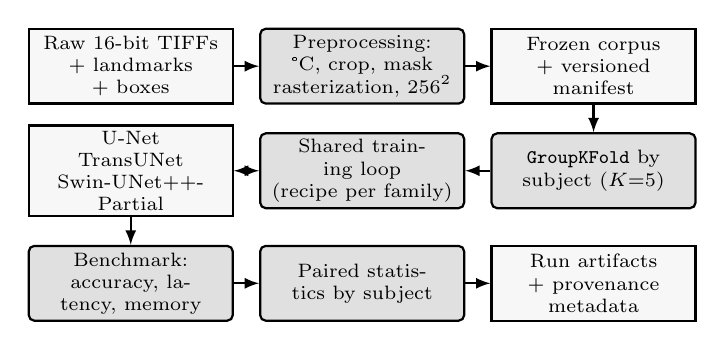
\begin{tikzpicture}[
  >=latex, thick,
  every node/.style={font=\scriptsize},
  proc/.style={rectangle, rounded corners=2pt, draw, fill=black!12, align=center, text width=2.45cm, minimum height=0.95cm, inner sep=2pt},
  art/.style={rectangle, draw, fill=black!3, align=center, text width=2.45cm, minimum height=0.95cm, inner sep=2pt},
  node distance=0.35cm and 0.32cm]
 \node[art]  (raw)  {Raw 16-bit TIFFs\\+ landmarks + boxes};
 \node[proc, right=of raw] (pre) {Preprocessing: \textdegree{}C, crop, mask rasterization, $256^2$};
 \node[art, right=of pre] (proc) {Frozen corpus\\+ versioned manifest};
 \node[proc, below=of proc] (cv) {\texttt{GroupKFold} by subject ($K{=}5$)};
 \node[proc, left=of cv] (train) {Shared training loop\\(recipe per family)};
 \node[art, left=of train] (models) {U-Net\\TransUNet\\\swinp};
 \node[proc, below=of models] (bench) {Benchmark: accuracy, latency, memory};
 \node[proc, right=of bench] (stats) {Paired statistics by subject};
 \node[art, right=of stats] (out) {Run artifacts\\+ provenance metadata};
 \draw[->] (raw) -- (pre); \draw[->] (pre) -- (proc); \draw[->] (proc) -- (cv);
 \draw[->] (cv) -- (train); \draw[<->] (train) -- (models);
 \draw[->] (models) -- (bench); \draw[->] (bench) -- (stats); \draw[->] (stats) -- (out);
\end{tikzpicture}
\caption{UBench pipeline. Rectangles: persisted artifacts; rounded boxes: processing stages.}
\label{fig:pipeline_ubench}
\end{figure}

%------------------------------------------------------------------------------
\subsection{Dataset and reference masks} \label{subsec:charlotte_thermalface}

Charlotte-ThermalFace \cite{Ashrafi2022} contains about 10{,}000 thermal face images of 10 subjects, acquired at ambient temperatures from $20.5$ to $26.5$\,\degC{} with varying humidity, air velocity, and capture distance, and stored as 16-bit raw radiometric frames.
After discarding unreadable frames, missing landmarks, and degenerate crops, the corpus has \textbf{8{,}074 images}.
The dataset provides anatomical \textbf{landmarks}, not segmentation masks; reference masks are therefore \textbf{derived}: each image is cropped around the face bounding box with a fixed margin, landmarks are shifted to the (border-clamped) crop origin, and the landmarks of each region are grouped into a closed polygon and rasterized, following the precedent of Joshi et al.~\cite{Joshi2022}.
The 10 classes are background, lower face contour, left and right eyebrows, nose, left and right eyes, mouth, lips, and forehead; left/right follow the observer's viewpoint.
The derivation code is deterministic and version-controlled, and the generated masks are frozen and verified by checksum.
Derived masks impose an architecture-independent \textbf{performance ceiling}: small regions bounded by few landmarks (eyebrows, lips) suffer proportionally larger polygonal approximation error, and no manual masks exist to quantify this noise.

%------------------------------------------------------------------------------
\subsection{Radiometric preprocessing and augmentation} \label{sec:preprocessamento_radiometrico}

Raw values (centikelvin) are converted to degrees Celsius and normalized using a \textbf{fixed} range, $[20, 40]$\,\degC{}$\,\mapsto[0,1]$, identical for all images.
The usual per-image min--max normalization would eliminate absolute temperature information, which is exactly what distinguishes thermography from a grayscale image; the fixed range preserves comparability across images and subjects, as advocated by \cite{Joshi2022}.
Images are resized to $256\times256$ with bilinear interpolation and masks with nearest neighbor.
A manifest records the schema version, unit, resolution, and normalization; the loader raises an explicit error if it is missing or incompatible, so data produced under an older convention cannot be silently reinterpreted.
Because pixel values are temperatures, photometric augmentations (brightness, contrast) are excluded.
Augmentation combines geometric transforms (horizontal flip and affine), applied jointly to image and mask, with physically plausible radiometric perturbations applied in \degC{}: an additive sensor offset of up to $\pm0.5$\,\degC{} and Gaussian noise.

%------------------------------------------------------------------------------
\subsection{Evaluated architectures} \label{sec:arquiteturas_avaliadas}

All architectures are trained from scratch on the thermal data only (Table~\ref{tab:arquiteturas}).
\textbf{U-Net} \cite{Ronneberger2015} follows the canonical topology (widths $64\!\rightarrow\!512$, 1024-channel bottleneck).
\textbf{TransUNet} \cite{Chen2021} uses a convolutional encoder, a ViT-B/16-style bottleneck (768-d embeddings, 12 blocks, 12 heads) with a learned absolute positional embedding, and a convolutional decoder from $H/16$ to full resolution.

\textbf{\swinp{}} retains a hierarchical encoder consistent with the Swin-T scale \cite{Liu2021Swin} ($d{=}96$, depths $[2,2,6,2]$, heads $[3,6,12,24]$, $8\times8$ windows, $4\times4$ patches with patch merging) but \textbf{does not reproduce} Swin-UNet++ \cite{Liu2021Materials}, hence its name (abbreviated \swint{} in tables).
Four simplifications were necessitated by the 6~GB GPU memory constraint: a Swin decoder with patch expanding, a full nested skip grid, and deep supervision would exceed the available memory budget at $256\times256$ without mixed precision, so the decoder is convolutional with collapsed nested skips and a $4\times$ interpolation from $H/4$.
Three additional omissions affect the attention mechanism itself: the shifted-window mask, the relative position bias, and any positional encoding.
Without them, window attention is permutation-invariant within each window.
Its results are therefore reported as a \textbf{simplified baseline}, not as evidence about Swin-style window attention.
Pre-trained variants (SwinV2-T and R50+ViT-B/16 from \texttt{timm}) exist in the pipeline but are excluded by design: mixing ImageNet-pretrained and from-scratch models would primarily reflect the effect of pre-training.

\begin{table}[tbp]
\centering
\caption{Evaluated architectures (none pre-trained)}
\label{tab:arquiteturas}
\footnotesize
\setlength{\tabcolsep}{3pt}
\begin{tabular}{@{}>{\raggedright\arraybackslash}p{1.55cm}>{\raggedright\arraybackslash}p{2.75cm}>{\raggedright\arraybackslash}p{2.35cm}r@{}}
\toprule
\textbf{Architecture} & \textbf{Encoder} & \textbf{Attention} & \textbf{Par.\,(M)} \\
\midrule
U-Net & Convolutional & None & 31.0 \\
TransUNet & Conv.\ + ViT-B/16 bottleneck & Global, at bottleneck & 105.7 \\
\swint{} & Hierarchical, Swin-T scale & Windowed, simplified & 40.9 \\
\bottomrule
\end{tabular}
\end{table}

%------------------------------------------------------------------------------
\subsection{Training protocol} \label{subsec:recipes_otimizacao}

\textbf{Subject-disjoint cross-validation.}
We use $K=5$ folds with \texttt{GroupKFold} grouped by subject identity; an automated test asserts that no subject appears in both training and validation of any fold.
Each subject is validated exactly once.
\texttt{GroupKFold} balances sample counts and is deterministic, yielding the validation pairs \{S2,S5\}, \{S8,S9\}, \{S6,S10\}, \{S3,S7\}, and \{S1,S4\} for folds 1--5.

\textbf{Family-specific recipes and budget.}
Imposing one optimizer and schedule on all families is not neutral; it is the poorly tuned baseline that \cite{Isensee2024} identify as a source of spurious conclusions.
Each family therefore uses its canonical recipe, without any hyperparameter search (Table~\ref{tab:hiperparametros}): the transformer family uses AdamW with decoupled weight decay \cite{Loshchilov2019}, linear warm-up, and cosine decay, as in \cite{Liu2021Swin}; U-Net uses Adam with \texttt{ReduceLROnPlateau}, the conventional setting for medical U-Nets \cite{Siddique2021}.
The budget is \textbf{100 epochs} for every architecture.
Batch sizes are selected by the hardware probe as the largest that fits in memory (8 for U-Net, 6 for the transformers), so the transformers perform about $33\%$ more weight updates per epoch (1{,}077 vs.\ 807); this asymmetry, like gradient clipping, favors the transformer family and is declared rather than hidden.
All models minimize $\mathcal{L}=0.5\,\mathcal{L}_{CE}+0.5\,\mathcal{L}_{Dice}$ \cite{Milletari2016,Sudre2017,Jadon2020} with uniform class weights.

\begin{table}[tbp]
\centering
\caption{Training hyperparameters by family}
\label{tab:hiperparametros}
\footnotesize
\setlength{\tabcolsep}{3pt}
\begin{tabular}{@{}lll@{}}
\toprule
 & \textbf{U-Net (CNN)} & \textbf{TransUNet, \swint{}} \\
\midrule
Optimizer & Adam & AdamW \\
Learning rate & $1{\times}10^{-4}$ & $1{\times}10^{-4}$ \\
Weight decay & $0$ & $0.05$ \\
Scheduler & Plateau (pat.\ 5, $\times0.5$) & 5\% warm-up $\rightarrow$ cosine \\
Grad.\ clipping & none & $1.0$ \\
Batch / epochs & 8 / 100 & 6 / 100 \\
\bottomrule
\end{tabular}
\end{table}

\textbf{Epoch selection.}
The \textbf{primary} result uses the model at the \textbf{final epoch} of the budget, fixed \textit{a priori} and independent of validation performance.
The \textbf{secondary} result uses the epoch with the best validation mIoU, which is optimistic by construction because the same partition selects and reports.
The plateau scheduler of U-Net is itself conditioned on validation mIoU, a mild adaptation that favors U-Net, i.e., acts against the main result.

%------------------------------------------------------------------------------
\subsection{Metrics and cost instrumentation} \label{subsec:metricas_acuracia}

\textbf{Accuracy.} mIoU and Dice are computed on argmax predictions from a single confusion-matrix implementation (\texttt{torchmetrics}) shared by the training loop and the benchmark module, which rules out silent discrepancies between two implementations of the same metric.
The per-image macro average excludes classes absent from the reference, and the background is reported separately.
Boundary metrics (HD95, NSD) are out of scope.

\textbf{Cost.} Latency discards 20 warm-up iterations, times 200, and explicitly synchronizes the GPU before reading the clock; otherwise one measures the asynchronous kernel queue rather than the computation.
Latency and peak memory use a \textbf{fixed batch of 4} for all architectures, since peak memory scales with batch size.
Only one model resides on the GPU, and \texttt{reset\_peak\_memory\_stats} and \texttt{max\_memory\_allocated} bracket the forward pass.
Three repetitions give identical values, and a fourth with 300~MB of unrelated tensors resident differs by less than 1~MB, so the measurement is independent of evaluation order.
We also report parameters, checkpoint size, and wall-clock training time per fold.

%------------------------------------------------------------------------------
\subsection{Statistical analysis} \label{sec:analise_estatistica}

Comparisons are \textbf{paired by subject}: each subject is evaluated once by a model that never saw it, giving $n=10$ paired observations per comparison.
We report mean differences, wins, the exact two-sided Wilcoxon signed-rank test, 95\% bootstrap confidence intervals of the paired differences (20{,}000 resamples), and Holm correction \cite{Holm1979}.
The pairing unit matters: the smallest attainable exact $p$-value is $2/2^{n}$, i.e., $0.0625$ when pairing by fold ($n=5$), above the 5\% threshold however consistent the folds are, but $\approx0.0020$ for $n=10$.
Because the two subjects of a fold share one trained model, subject-level $p$-values are slightly optimistic, so fold-level pairing ($n=5$ independent models) is reported as a secondary analysis.

%------------------------------------------------------------------------------
\subsection{Execution environment and pipeline audit} \label{subsec:auditoria_defeitos}

The reported run used one NVIDIA GTX~1660~Ti (6~GB), PyTorch~2.5.1 with CUDA~12.1, seed~42 with deterministic mode, and no mixed precision (unsupported on this GPU class), totaling \textbf{186.9 GPU-hours} for the 15 architecture--fold combinations.
The run was launched from a working tree with uncommitted changes outside the pipeline code; the source tree is byte-identical to the tagged commit, and the difference is versioned as a patch, so the run is reproducible from a commit plus an inspectable patch.
Before the run, the pipeline underwent a systematic audit.
Overall, \textbf{32 issues} were cataloged: 26 found by the pre-run audit, four revealed by the pattern of the results (UB-27 to UB-30), and two by verifying the corrections; 28 are corrected and verified, mostly by automated regression tests, and four are disclosed exceptions (e.g., UB-17, the attention omissions of \swinp{}).
The pre-run classes covered divergent metric definitions, partition integrity, preprocessing and architectural fidelity, efficiency measured under unequal conditions, and environment drift.
Issues relevant to interpreting the results are discussed where they arise.


%==============================================================================
\section{Results} \label{sec:resultados}
%==============================================================================

All figures come from a single identified run of the pipeline; trained weights, per-epoch histories, and per-fold metrics are preserved.
No subject was held out for testing, so all accuracy metrics are \textbf{validation} metrics, each subject being evaluated by the model of the fold in which it was not trained.
The three architectures completed the 100-epoch budget in all folds without divergence or severe overfitting, so neither the budget nor the family recipes were inadequate for any architecture.

%------------------------------------------------------------------------------
\subsection{Accuracy and statistical significance} \label{sec:res_acuracia}

Table~\ref{tab:comparacao_acuracia} reports both epoch-selection variants.
The best-epoch variant exceeds the final-epoch one for every architecture, as expected from selecting and reporting on the same partition.
In both variants and in all five folds the ranking is TransUNet $>$ U-Net $>$ \swinp{}, with no inversion.
Dice is below $2\,\mathrm{mIoU}/(1+\mathrm{mIoU})$ in every cell, as Jensen's inequality requires when both metrics are computed per class from the same predictions before averaging.
Fig.~\ref{fig:qualitativa_comparacao} shows predictions for samples chosen by quantitative criteria, each predicted with final-epoch weights by the model of the fold in which its subject was validated.

\begin{figure}[tbp]
\centering
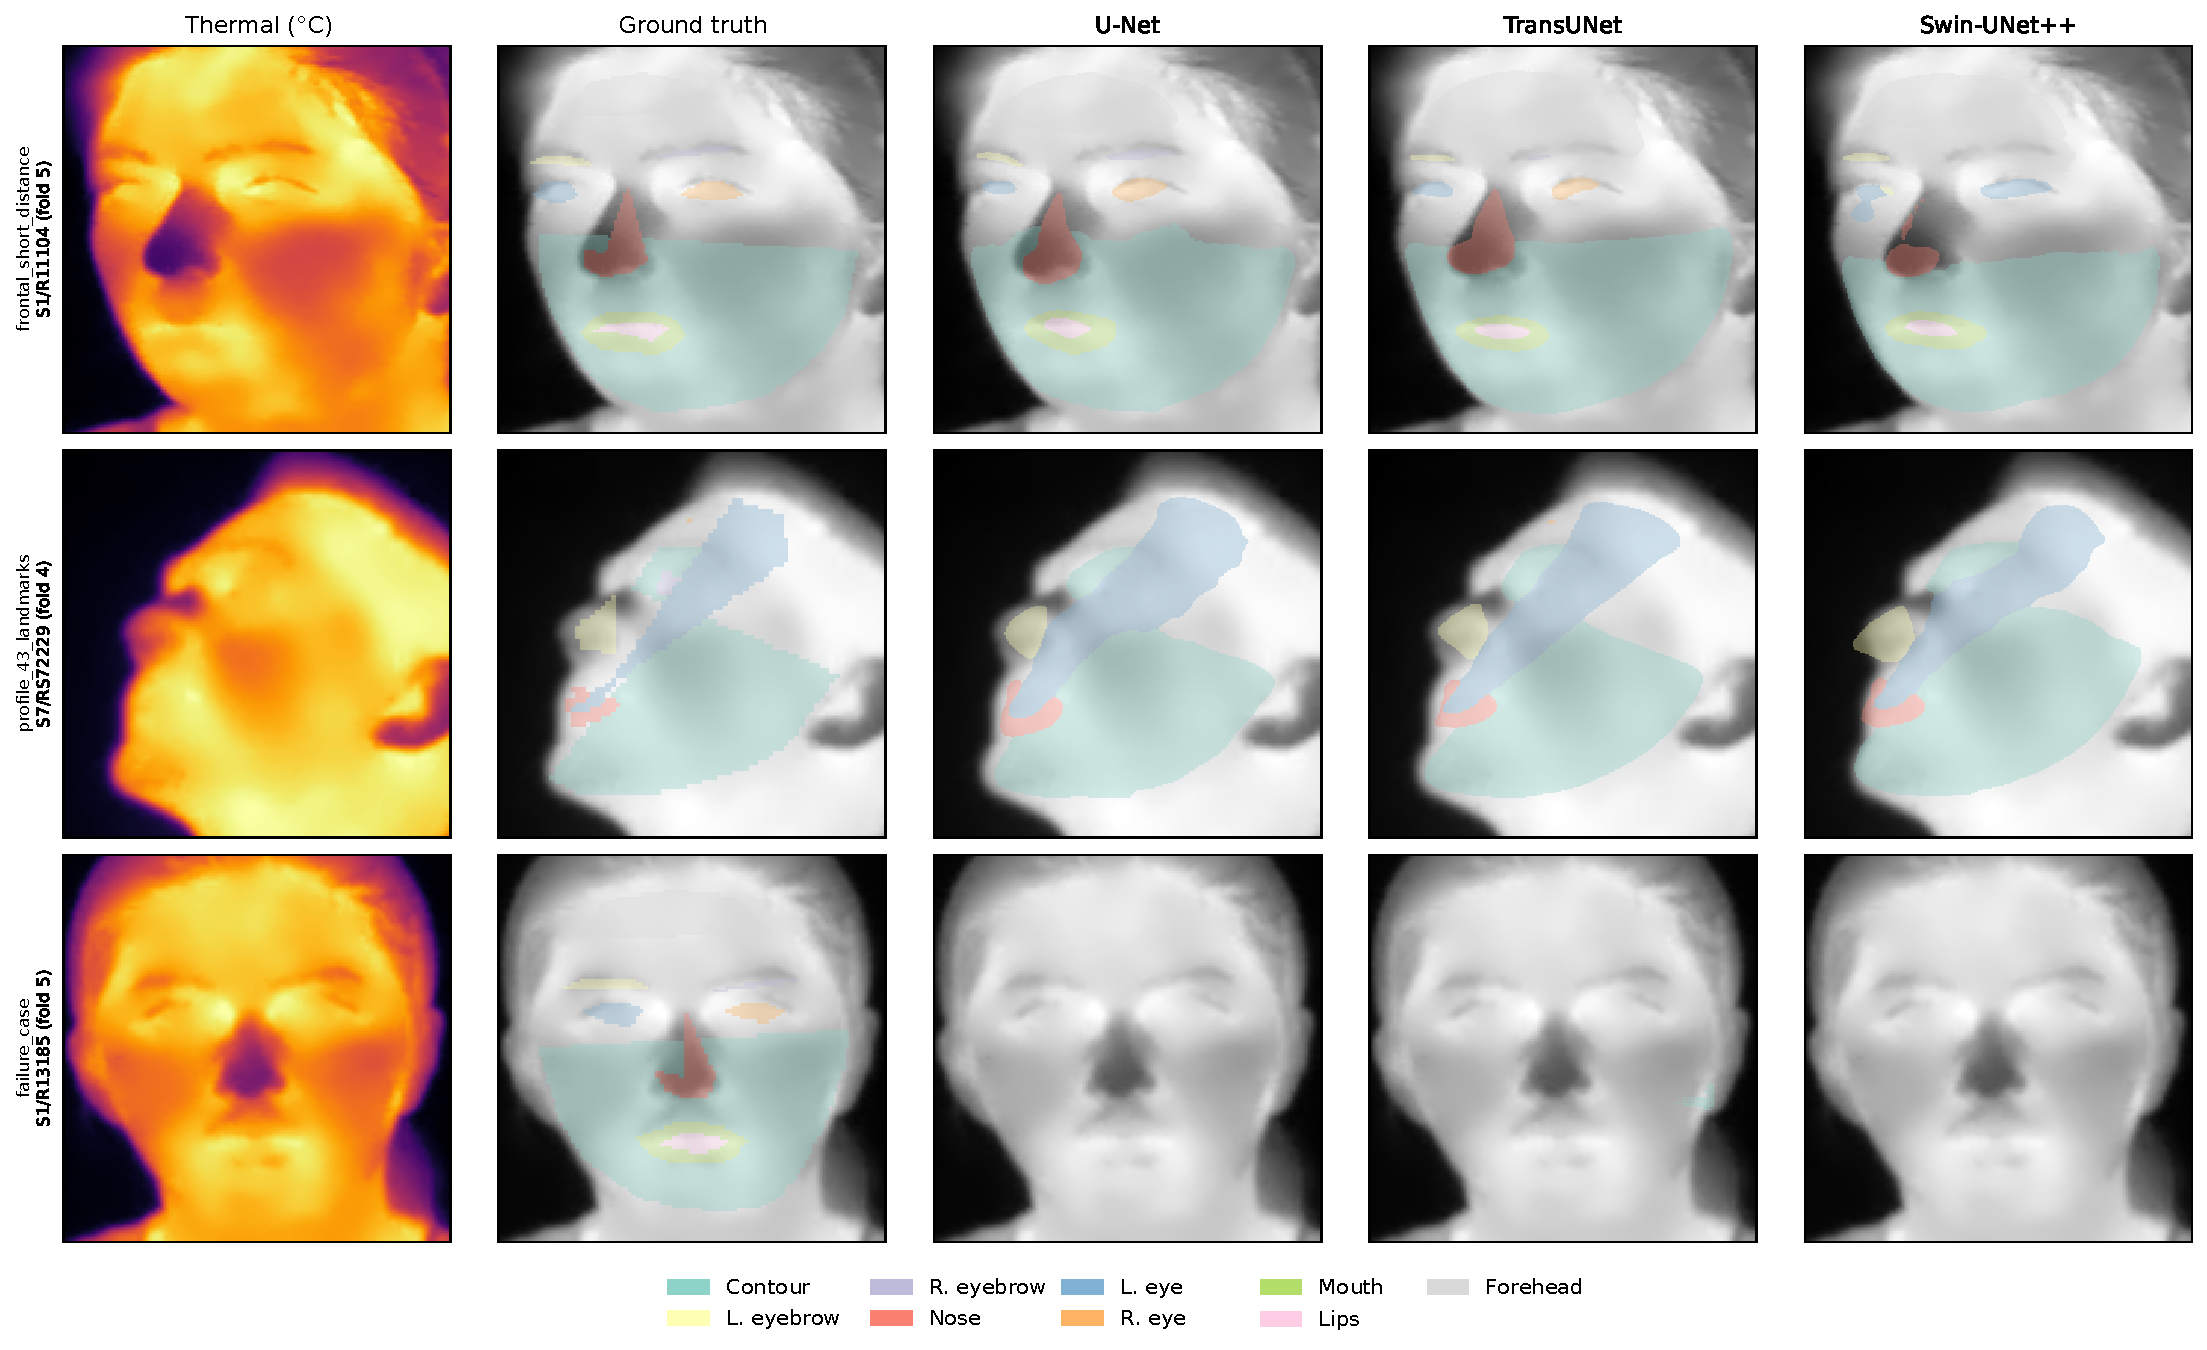
\includegraphics[width=\columnwidth]{img/resultados/fig_qualitativa-1.pdf}
\caption{Qualitative comparison. Columns: thermal image, derived reference, U-Net, TransUNet, \swint{}. Rows: closest annotated capture distance (frontal); median-performance profile view, showing the displaced ``left eye'' of Section~\ref{subsec:res_anomalia_lateral}; lowest-mIoU validation sample.}
\label{fig:qualitativa_comparacao}
\end{figure}

\begin{table}[tbp]
\centering
\caption{Accuracy (mean $\pm$ std.\ across the five folds)}
\label{tab:comparacao_acuracia}
\footnotesize
\setlength{\tabcolsep}{3pt}
\begin{tabular}{@{}lccc@{}}
\toprule
& \multicolumn{2}{c}{\textbf{Final epoch (primary)}} & \textbf{Best epoch} \\
\cmidrule(lr){2-3}\cmidrule(lr){4-4}
\textbf{Architecture} & \textbf{mIoU} & \textbf{Dice} & \textbf{mIoU} \\
\midrule
TransUNet & $\mathbf{0.4333 \pm 0.0491}$ & $\mathbf{0.5910}$ & $\mathbf{0.4471 \pm 0.0493}$ \\
U-Net & $0.4045 \pm 0.0527$ & $0.5599$ & $0.4191 \pm 0.0548$ \\
\swint{} & $0.3529 \pm 0.0430$ & $0.4978$ & $0.3743 \pm 0.0456$ \\
\bottomrule
\end{tabular}
\end{table}

Table~\ref{tab:comparacoes_pareadas} tests whether this ordering is distinguishable from experimental variability.
Under subject pairing, all three comparisons are significant, the bootstrap intervals exclude zero, and the Holm-adjusted $p$-value is $0.0059$ for each.
Fold pairing, with the same sign in 15 of 15 cases, cannot reach significance because its floor is $0.0625$.
Two of the three comparisons sit exactly at the floor of the $n=10$ test, so they are as significant as the design permits, and no more.
The subject-level view also reveals heterogeneity hidden by folds: TransUNet beats U-Net on 9 of 10 subjects, the exception being S6.

\begin{table}[tbp]
\centering
\caption{Paired comparisons of final-epoch mIoU}
\label{tab:comparacoes_pareadas}
\footnotesize
\setlength{\tabcolsep}{2.5pt}
\begin{tabular}{@{}lcccc@{}}
\toprule
\textbf{Comparison} & \textbf{$\Delta$mIoU} & \textbf{Wins} & \textbf{Wilcoxon $p$} & \textbf{95\% CI} \\
\midrule
\multicolumn{5}{@{}l}{\textit{Paired by subject ($n=10$), primary}} \\
TransUNet -- U-Net & $+0.0296$ & 9/10 & $\mathbf{0.0039}$ & $[0.016, 0.045]$ \\
U-Net -- \swint{} & $+0.0573$ & 10/10 & $\mathbf{0.0020}$ & $[0.036, 0.078]$ \\
TransUNet -- \swint{} & $+0.0868$ & 10/10 & $\mathbf{0.0020}$ & $[0.064, 0.110]$ \\
\midrule
\multicolumn{5}{@{}l}{\textit{Paired by fold ($n=5$), secondary}} \\
TransUNet -- U-Net & $+0.0288$ & 5/5 & $0.0625$ & $[0.019, 0.041]$ \\
U-Net -- \swint{} & $+0.0517$ & 5/5 & $0.0625$ & $[0.042, 0.064]$ \\
TransUNet -- \swint{} & $+0.0805$ & 5/5 & $0.0625$ & $[0.068, 0.093]$ \\
\bottomrule
\end{tabular}
\end{table}

%------------------------------------------------------------------------------
\subsection{Partition variability versus architecture effect} \label{subsec:res_variabilidade_particoes}

Averaging the three architectures within each fold measures the \textbf{difficulty of each partition}.
It ranges from $0.3444$ (fold 2) to $0.4439$ (fold 5), a spread of $\mathbf{0.0995}$, larger than the largest mean difference between architectures ($0.0868$, TransUNet vs.\ \swinp{}).
\textbf{Which subjects form the validation partition affects the measured mIoU more than the choice of architecture}, even between the best and the worst of the three.
A single train/test split would thus have yielded an estimate, and possibly a ranking, that depended on which subjects happened to be drawn.
A competing explanation is view composition: fold 2 has the largest share of profile views ($61.8\%$), whose masks are defective (Section~\ref{subsec:res_anomalia_lateral}).
The explanation does not survive stratification: restricted to frontal views, the hardest fold becomes fold 3 (U-Net $0.3788$ vs.\ $0.4109$ for fold 2), driven by subject S10, whose mIoU ($0.166$--$0.194$) is $4.15$ standard deviations below the other nine.
Fold ordering is explained by subject identity rather than by view composition.

%------------------------------------------------------------------------------
\subsection{Per-class performance and the lateral anomaly} \label{subsec:res_anomalia_lateral}

Table~\ref{tab:iou_por_classe} reports per-class IoU.
Large regions (background, lower contour, forehead) score highest in all architectures.
Across the nine foreground classes, mean IoU correlates with class area in the processed corpus (Spearman $\rho=+0.900$, $p=0.0009$), but only moderately and non-significantly with the area measured on frontal views, which are free of the defect described below ($\rho=+0.633$, $p=0.067$).
Area is thus a strong but not dominant factor; mask fidelity acts in the same direction.

\begin{table}[tbp]
\centering
\caption{Per-class IoU (best epoch, aggregated over folds)}
\label{tab:iou_por_classe}
\footnotesize
\setlength{\tabcolsep}{4pt}
\begin{tabular}{@{}lccc@{}}
\toprule
\textbf{Class} & \textbf{U-Net} & \textbf{TransUNet} & \textbf{\swint{}} \\
\midrule
Background & 0.8826 & 0.8976 & 0.8884 \\
Lower face contour & 0.7162 & 0.7623 & 0.7342 \\
Left eyebrow\textsuperscript{\textdagger} & 0.4176 & 0.4285 & 0.3288 \\
Right eyebrow\textsuperscript{\textdagger} & 0.3012 & 0.3213 & 0.1931 \\
Nose & 0.3771 & 0.4150 & 0.3359 \\
Left eye\textsuperscript{\textdagger} & 0.4958 & 0.5194 & 0.4788 \\
Right eye\textsuperscript{\textdagger} & 0.4190 & 0.4314 & 0.2325 \\
Mouth & 0.2891 & 0.3225 & 0.2983 \\
Lips & 0.2666 & 0.3104 & 0.2800 \\
Forehead & 0.4891 & 0.5133 & 0.4875 \\
\bottomrule
\multicolumn{4}{@{}l}{\textsuperscript{\textdagger}\,Lateralized classes affected by UB-27 and UB-30.}
\end{tabular}
\end{table}

\textbf{Observation.} Anatomically equivalent classes differ systematically by side: left exceeds right by $0.107$--$0.136$ IoU for eyebrows and $0.077$--$0.246$ for eyes.
Faces are roughly symmetric and no architecture favors one side of the image, so a gap that persists in all three architectures and all folds points to the \textbf{data}.
Two independent defects, both discovered from this pattern and missed by the pre-run audit, produce it.

\textbf{UB-27: landmark scheme resolved from the file header.}
The dataset annotates 73 landmarks on frontal views and 43 on profile views, but every annotation file declares 73 columns for all rows, and the code chose the scheme from the header.
Profile rows (50.0\% of the corpus) were therefore read with the 73-point mapping: mouth, lips, and forehead vanish from their reference, the right eye collapses to a vestigial vertex (19~px on average vs.\ 414~px on frontal views), and the left eye receives a large, displaced polygon (6{,}131~px vs.\ 429~px) built from points that belong to the lips and forehead (Fig.~\ref{fig:anomalia_lateral_visual}).
On profile views, the macro average thus covers about six classes instead of nine.

\textbf{UB-30: horizontal flip without label permutation.}
Since labels follow the observer's side, flipping moves a structure across the facial midline without swapping its label.
With flip probability $0.5$, ``left'' and ``right'' were assigned to both halves of the face, so for the four lateralized classes the label ceased to be a function of the image.
The fix, a label permutation performed atomically with the flip, is implemented and tested, but was not applied retroactively.

\begin{figure}[tbp]
\centering
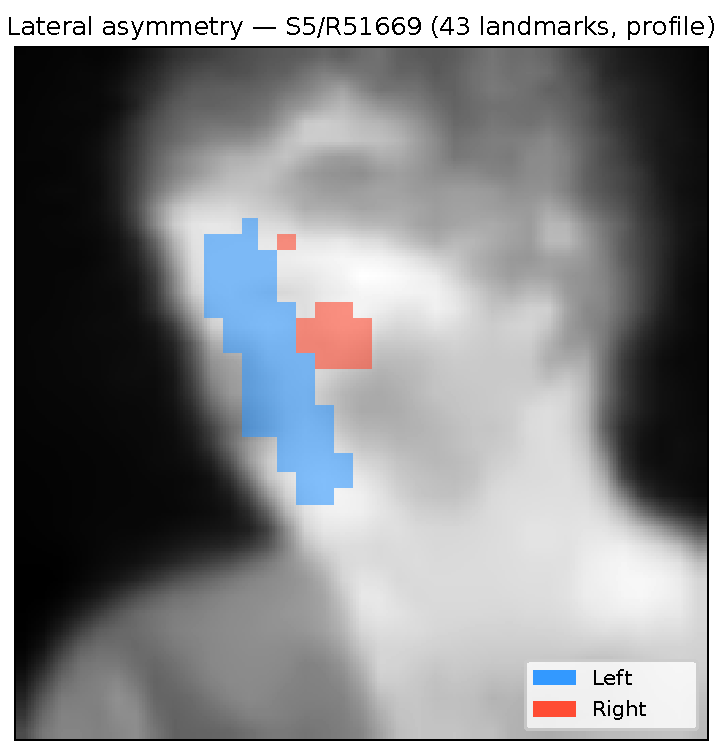
\includegraphics[width=0.48\columnwidth]{img/resultados/fig_anomalia_lateral-1.pdf}
\caption{Profile view with the derived lateral regions overlaid: the ``left eye'' (blue) is large and displaced; the ``right eye'' (red) is reduced to a vestige.}
\label{fig:anomalia_lateral_visual}
\end{figure}

\textbf{Robustness to the affected classes.}
Excluding the four lateralized classes (best-epoch aggregate), U-Net and \swinp{} differ by only $+0.0004$, whereas within those four classes U-Net leads by $+0.1001$: its whole advantage lies in classes whose labels were not a function of the image.
To test this, the 15 preserved final-epoch checkpoints were re-evaluated per subject, without retraining, on the macro of the five non-lateralized classes (Table~\ref{tab:comparacoes_5classes}).
TransUNet remains significantly ahead of both models even after Holm correction, while U-Net vs.\ \swinp{} becomes $+0.0040$ with 5/10 wins and $p=0.77$.
The robust answer to RQ1 is therefore the \textbf{partial ordering} TransUNet $>$ \{U-Net, \swinp{}\}.

\begin{table}[tbp]
\centering
\caption{Subject-paired comparisons on the five non-lateralized classes ($n=10$)}
\label{tab:comparacoes_5classes}
\footnotesize
\setlength{\tabcolsep}{3pt}
\begin{tabular}{@{}lcccc@{}}
\toprule
\textbf{Comparison} & \textbf{$\Delta$mIoU} & \textbf{Wins} & \textbf{Wilcoxon $p$} & \textbf{Holm} \\
\midrule
TransUNet -- U-Net & $+0.0437$ & 9/10 & $\mathbf{0.0039}$ & $\mathbf{0.0078}$ \\
U-Net -- \swint{} & $+0.0040$ & 5/10 & $0.7695$ & $0.7695$ \\
TransUNet -- \swint{} & $+0.0477$ & 10/10 & $\mathbf{0.0020}$ & $\mathbf{0.0059}$ \\
\bottomrule
\end{tabular}
\end{table}

\textbf{Ablation of UB-30.}
A second run, identical in seed, partitions, recipes, budget, and masks except for the flip fix, isolates UB-30.
On the five non-lateralized classes, \swinp{} rises from $0.4272$ to $0.4363$ and \textbf{overtakes} U-Net ($0.4266$), reversing the sign of their difference; TransUNet stays ahead in all folds.
On the four lateralized classes, however, \swinp{} drops from $0.3083$ to $0.2573$: under UB-27 the displaced polygon was consistently labeled ``left eye'' and hence learnable, whereas with permutation it alternates between labels.
Fixing one defect while leaving the other in place worsens the classes affected by both, so the two corrections must be applied together.
The corrected derivation (per-image scheme and visible side inferred from landmark geometry) has been verified on the full corpus but not yet used for retraining; absolute mIoU values are therefore a likely \textbf{lower bound}.

%------------------------------------------------------------------------------
\subsection{Computational efficiency} \label{sec:res_eficiencia}

Table~\ref{tab:custo_computacional} reports cost under the equalized conditions of Section~\ref{subsec:metricas_acuracia}.
\textbf{The speed ordering reverses the accuracy ordering}: \swinp{} is $1.6\times$ faster than U-Net and $2.3\times$ faster than TransUNet, uses the least inference memory, and trains $2.2\times$ faster per fold.
Although it has more parameters than U-Net ($40.9$~M vs.\ $31.0$~M), it uses about half the memory, because under a fixed batch peak memory is dominated by intermediate activations, which depend on the spatial resolutions kept through the network, not by weights.
Fig.~\ref{fig:fronteira_compromisso} summarizes the trade-off (RQ3): no architecture dominates; TransUNet maximizes accuracy at the highest latency and model size, \swinp{} minimizes cost at the lowest accuracy, and U-Net lies in between.

\begin{table}[tbp]
\centering
\caption{Computational cost (fixed batch of 4, GTX 1660 Ti)}
\label{tab:custo_computacional}
\footnotesize
\setlength{\tabcolsep}{2.5pt}
\begin{tabular}{@{}lcccccc@{}}
\toprule
\textbf{Arch.} & \textbf{ms/img} & \textbf{img/s} & \textbf{Peak (MB)} & \textbf{Size (MB)} & \textbf{Par.\,(M)} & \textbf{Train/fold} \\
\midrule
U-Net & 17.99 & 55.6 & 555.9 & 118.4 & 31.04 & 921.7 min \\
TransUNet & 25.53 & 39.2 & 591.7 & 403.2 & 105.71 & 908.7 min \\
\swint{} & \textbf{11.15} & \textbf{89.7} & \textbf{300.6} & 156.1 & 40.92 & \textbf{413.0} min \\
\bottomrule
\end{tabular}
\end{table}

\begin{figure}[tbp]
\centering
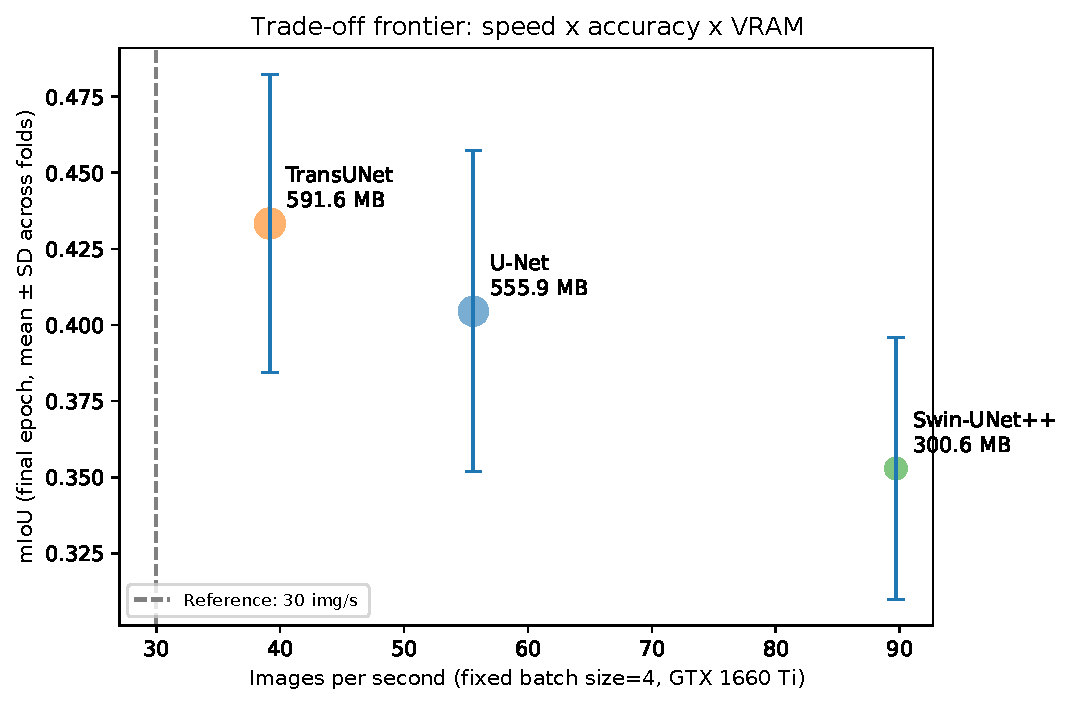
\includegraphics[width=0.92\columnwidth]{img/resultados/fig_pareto-1.pdf}
\caption{Accuracy--throughput trade-off. Error bars: $\pm1$ std.\ across folds; labels give peak inference memory (fixed batch of 4).}
\label{fig:fronteira_compromisso}
\end{figure}

\textbf{Two inversions of the memory ranking.}
Memory was measured incorrectly twice, and each error produced a different ranking.
The first measurement compared architectures under different batch sizes (UB-10) and ranked U-Net as the \textbf{most} memory-hungry.
The second fixed the batch but read the device-wide peak counter with all three models resident, so each was charged for the memory of those probed before it ($+30.9$, $+325.5$, and $+636.5$~MB).
It reported $586.7$, $917.1$, and $937.1$~MB, ranking U-Net as the \textbf{least} and \swinp{} as the most memory-hungry.
Only the isolated probe (UB-28) yields the values in Table~\ref{tab:custo_computacional}.
Latency had the same structural flaw, being originally measured under the per-architecture training batch sizes.

%------------------------------------------------------------------------------
\subsection{Capture distance} \label{sec:res_distancia}

Stratifying per-image mIoU by the quartiles of the annotated capture distance ($1.0$--$6.6$~m for $98.5\%$ of the corpus) shows no monotonic degradation.
All three architectures peak in the $2.8$--$4.0$~m range (e.g., TransUNet $0.457$ vs.\ $0.405$ at $1.0$--$1.8$~m), the architecture ranking holds in every range, and the peak persists when frontal and profile views are analyzed separately.
The within-range standard deviation ($0.12$--$0.16$) is two to three times the largest between-range difference ($0.05$).
Because faces are cropped and resized to $256\times256$, the apparent-size effect of distance is removed, and only blur and signal-to-noise effects remain; within the covered range, distance is not a dominant determinant of performance.


%==============================================================================
\section{Discussion} \label{sec:discussao}
%==============================================================================

\textbf{What the ordering does and does not say.}
Following \cite{Isensee2024}, we only grant a mechanistic explanation to differences that are significant under subject pairing and whose bootstrap interval excludes zero, and every explanation must still face two confounders declared before the analysis.
\textbf{Capacity}: TransUNet has $3.4\times$ the parameters of U-Net and also performs about $33\%$ more updates per epoch, which suffices to explain its lead without invoking any property of self-attention.
The result does say something narrower: training a ViT bottleneck from scratch on a few thousand images, often considered unfavorable, did not prevent it from converting extra capacity into accuracy.
\textbf{Fidelity}: \swinp{} informs about this baseline, not about Swin.
Between U-Net and \swinp{}, the difference dissolves once the lateralized classes are excluded, and the UB-30 ablation reverses its sign, so no architectural explanation is warranted.
As a hypothesis only, \swinp{} is the only model that discards positional information without restoring it (U-Net preserves it through translation-equivariant convolutions and skips; TransUNet has a learned positional embedding), and it degrades most where the discriminative cue is positional: telling left from right between near-identical structures.
The competing reading, that a weaker baseline degrades more where the task is harder, fits the data equally well.

\textbf{Comparison with the literature.}
Our best final-epoch mIoU ($43.3\%$) is about 24 points below the lowest value reported by Joshi et al.~\cite{Joshi2022} ($67.6$--$82.9\%$).
Six protocol differences separate the numbers, and five of them work against this study: nine times fewer subjects (10 vs.\ 90) with variable distance; five subject-disjoint folds instead of one 85/15 split; no pre-training; a fixed CE+Dice loss, whereas the loss alone moved their U-Net by $13.8$ points; and defective masks on half of the corpus.
The sixth, a different class scheme, has an undetermined direction.
No single difference explains the gap, and we do not isolate their contributions; absolute values should not be compared across these protocols.

\textbf{Lessons for benchmarking.}
Most of the 32 audited issues raised no error at all; they silently degraded results, several producing numbers plausible enough to publish.
Three lessons generalize beyond this domain.
\emph{(1) Agreement with theory is not validation.} The second, non-isolated memory probe agreed with the intuition that more parameters means more memory, and that agreement was taken as evidence that the instrument was correct; a partial fix (equal batches) also closed the investigation prematurely.
Cost measurements need their own controls: fixed batch, explicit synchronization, warm-up exclusion, probe isolation, and a perturbation test.
\emph{(2) Code reading has two blind spots.} UB-27 lived in the relation between code and data format, not in any single file, while UB-30 was visible in a single file but required the reviewer to hold the right semantic premise in mind.
Measurement on artifacts catches the first kind of issue; metamorphic tests that encode domain invariants, such as ``flipping must swap lateral labels'', catch the second without prior suspicion of a defect, and validating each implementation against its published result would have exposed the omissions in \swinp{} before any run.
\emph{(3) Fixing code does not fix artifacts.} A later run that already contained the mask fix produced byte-identical defective masks, because two serial caches (UB-31) skipped regeneration; tests passed legitimately.
Only measuring the quantity that the defect distorted, here the lateral asymmetry, revealed that the fix had not been materialized.

\textbf{Threats to validity.}
\emph{Construct}: masks are derived from landmarks, with no inter-annotator reference; boundary metrics are not computed; and UB-27/UB-30 bias the lateralized classes, which is why we report the partial ordering.
\emph{Internal}: capacity is not matched, the budget is equalized in epochs rather than steps or time, and the U-Net scheduler is conditioned on validation mIoU.
\emph{External}: one dataset with 10 subjects, one sensor and acquisition protocol, one GPU, and no external baseline such as nnU-Net \cite{Isensee2021}; the ranking concerns these implementations only.
\emph{Conclusion}: a single seed, so variance is across partitions rather than seeds; two subjects share each trained model; two comparisons sit at the test floor; and there is no held-out test set.


%==============================================================================
\section{Conclusion} \label{sec:conclusao}
%==============================================================================

We presented UBench, an open benchmarking framework for multi-region semantic segmentation of thermal faces in which all architectures share the training loop, metric implementation, and cost instrumentation, and we used it to compare U-Net, TransUNet, and \swinp{} on Charlotte-ThermalFace under subject-disjoint cross-validation, family-specific recipes, an identical budget, and subject-paired tests.
TransUNet is the most accurate architecture (RQ1), but the robust claim is the partial ordering TransUNet $>$ \{U-Net, \swinp{}\}, because the U-Net advantage over \swinp{} is confined to classes corrupted by mask-derivation and augmentation defects.
Per-class IoU grows with region area, an association that weakens where masks are correctly derived (RQ2).
Under equalized measurement, efficiency reverses accuracy (RQ3): \swinp{} delivers $89.7$ images/s with $300.6$~MB, against $39.2$ images/s and $591.7$~MB for TransUNet.
Above all, the spread across validation partitions exceeds the largest architectural difference, independent evidence in this domain for the critique of loosely controlled architecture comparisons \cite{Isensee2024}.

Future work includes retraining with both corrections applied together, adding nnU-Net and pre-trained encoders as external anchors, computing boundary metrics, holding out test subjects, and validating the framework on a second thermal dataset.
Code, configuration, trained weights, and per-fold and per-subject metrics are available in an anonymized repository for review.
% TODO before submission: add the Anonymous GitHub link here (e.g., \url{https://anonymous.4open.science/r/...}).
% Camera-ready: replace with the public repository and the Zenodo DOI.


\bibliographystyle{ieeetran}
\bibliography{bibliografia}

\end{document}